\chapter{Evaluation}\label{ch: Design}

This chapter evaluates the implementation of heterogeneity model as described in chapter \ref{ch:Implementation}. We will base our test data obtained from Cooja simulator log outputs. Cooja is a network simulator, which allows execution of TinyOS compiled codes in a virtual Telosb \ac{WSN} set up. Using the simulator, we can debug the model using print statements. These statements are displayed in Cooja \textit{mote output} window along with the time-stamp and sender id of debug statements. Cooja log files can be saved as \textit{.txt} files and therefore could be further used to obtain relevant visualisations and numerical calculations using statistical programming language such as \textit{R}.  

\par
In the first section of this chapter, we will explain the structure of test results obtained from the heterogeneity model along with the result analysis and in the second section we will evaluate our model for the five goals: reliability, robustness, fairness, efficiency and hardware independence.

%************************************************
\section{Structure and Analysis of Test Results}
%************************************************

To compare the analytical results with simulations (using Cooja), we use the network topologies as shown in figures \ref{fig:EllipsoidTopology} and \ref{fig:treeTopology}. Since, the size of the topology, the number of nodes deployed and number of nodes present in the \ac{PC} neighborhood can have significant impact on the protocol behaviour, we have focused on two important scenarios: 

\begin{enumerate}
    \item Frequent one hop data transmission: Demonstrated using \ref{fig:treeTopology}.
    
    \item Increased chances of two hop transmission: Demonstrated using \ref{fig:EllipsoidTopology}
    
\end{enumerate}

 \par
Figure \ref{fig:treeTopology} describes the tree arrangement of \acp{SN} in which the parent nodes three and five act as the \acp{PC}. We have also added eight as the shared \ac{PC} between the children of other two \acp{PC}. The reason for choosing this kind topology is to see how heterogeneity behaves in cases of frequent one hop data transmissions. We use another arrangement of \ac{SN} in an ellipsoidal pattern (as shown in figure \ref{fig:EllipsoidTopology}). In this topology, we have placed all the \ac{SN} in a ring like arrangement in which a \acp{SN} has exactly two neighbors in the one hop neighborhood. This network of \acp{SN} provides us more opportunities to observe more two hop data transmission requests than the tree topology because in this topology there can be maximum two nodes competing for one hop data transmission request where as in the tree topology we have more than two nodes competing for each of the \acp{PC}.

In the next subsections we will focus on the results obtained by simulating the heterogeneity model on these topologies in Cooja simulator at different heterogeneity data transfer rates. 

        \begin{figure}
        \centering
        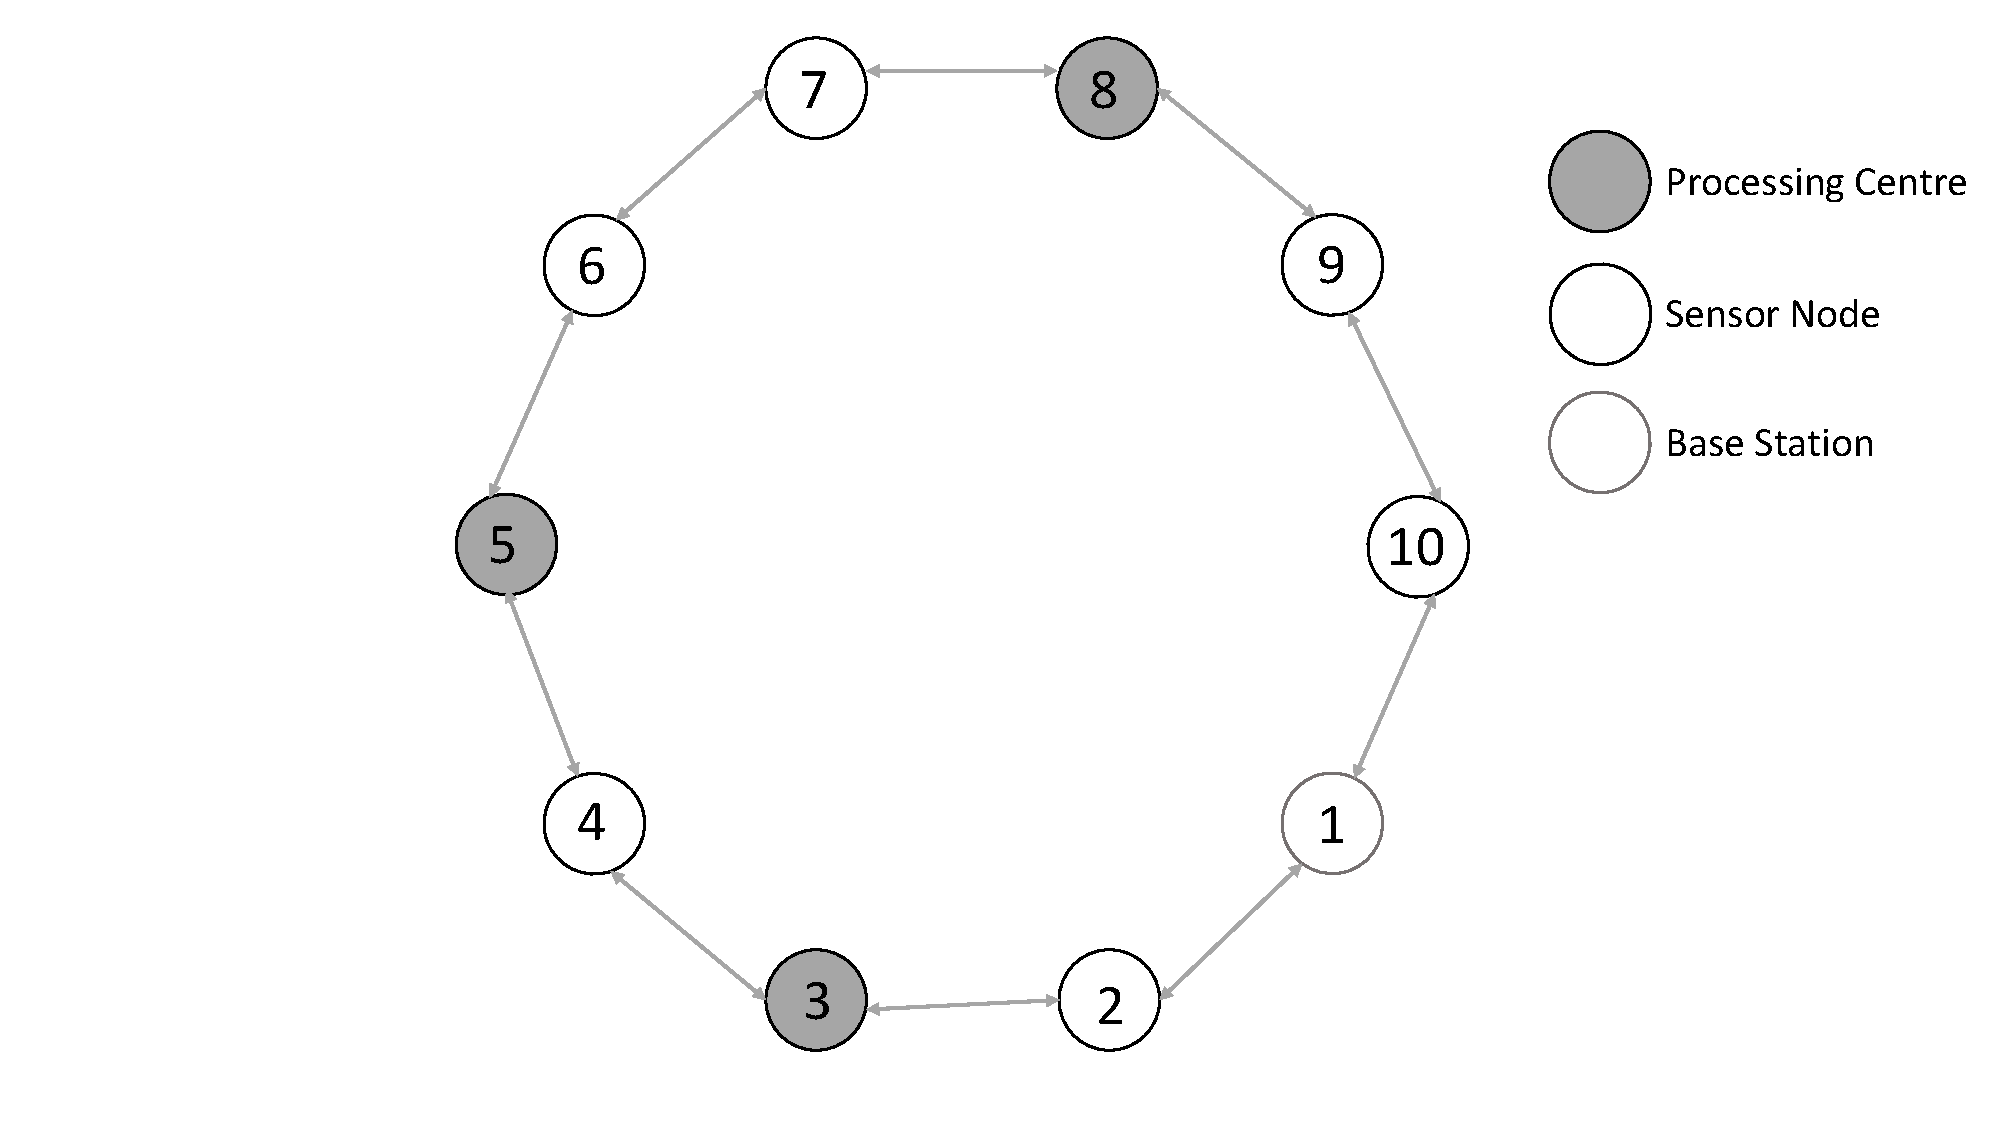
\includegraphics[width=1.0\textwidth]{gfx/RPlots/Ellipsoid_topology.pdf}
        \caption{Ellipsoid Topology}
        \label{fig:EllipsoidTopology}
        \end{figure}
        	
        \begin{figure}
        \centering
        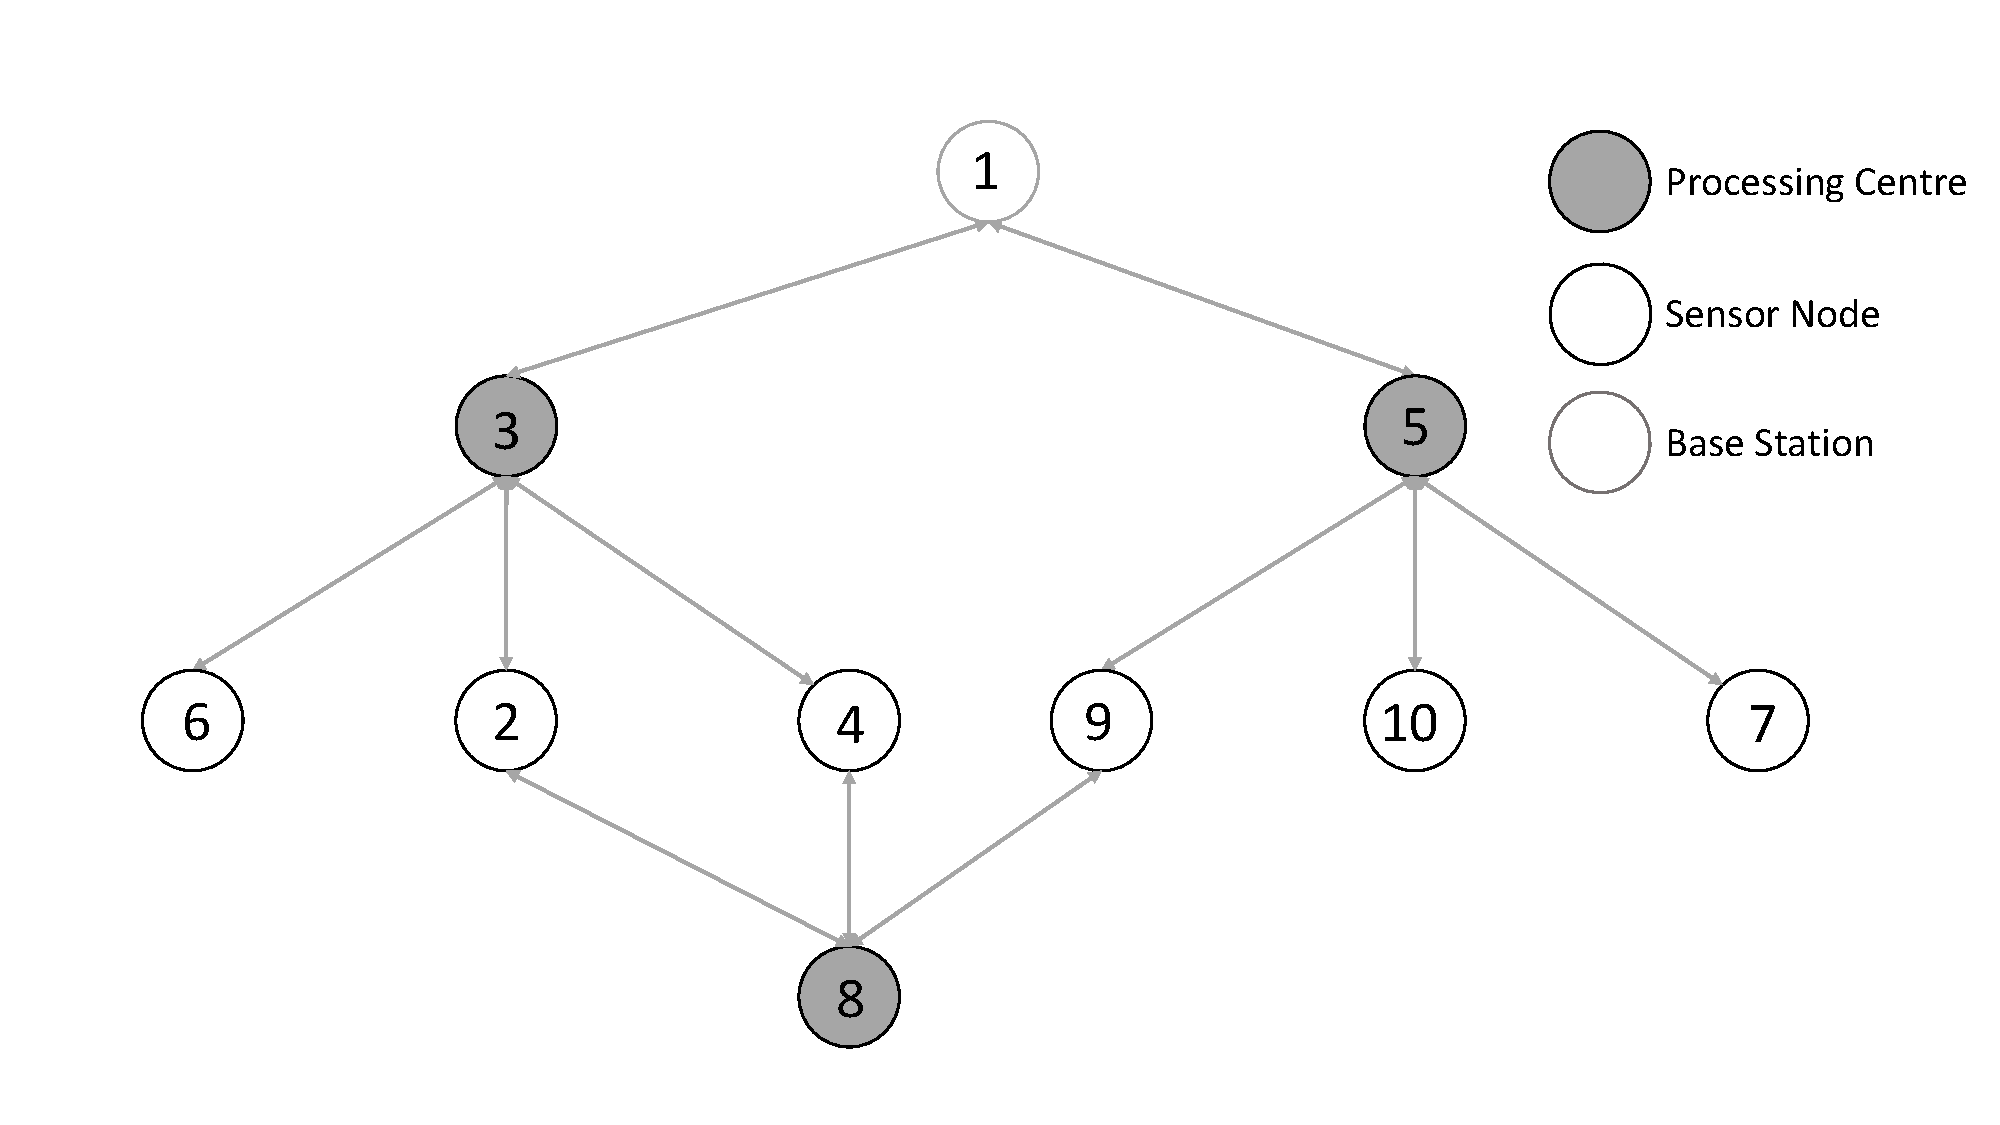
\includegraphics[width=1.0\textwidth]{gfx/RPlots/Tree_topology.pdf}
        \caption{Tree Topology}
        \label{fig:treeTopology}
        \end{figure}
        
    %************************************************
    \subsection*{Sender Enqueue-Dequeue Log}
    %************************************************
        
        It stores addresses of sender, relayer and \ac{PC} participating in the data transmission phase of the heterogeneity model. This information is printed using Cooja simulator. The simulator also provides the time-stamp for each of the debug statements. This feature is used to calculate the duration of data transfer between participating \acp{SN} and further plot a data transfer schedule to visualise the occupancy of available \acp{PC} during the data transmission phase \cite{bitencourt2012simulation}. 
        
        The figures \ref{fig:dfd_ellipsoid}, \ref{fig:dfd_tree} show the data transfer schedules of the intended senders in ellipsoid (\ref{fig:EllipsoidTopology}) and tree (\ref{fig:treeTopology}) topology respectively for approximately one hour simulation run time. It was difficult to plot more than one hour of simulation run time because of memory constraints. The Cooja simulator runs out of memory on simulating large number of nodes more more than one hour in our experiment.
        
        \par
        The simulation parameters used to plot these diagrams are explained as follows:
        
        \begin{enumerate}
            \item In the virtual environment scenario using Cooja simulator, we have selected \ac{UDGM} of data transmission. In this model of data transmission, all the \acp{SN} outside the $100units$ radius of a \ac{SN} do not receive any packets at all whereas the \acp{SN} within the sensor radius receive all the packets.
            
            \item In both the topologies, \acp{SN} with addresses three, five and eight are the\acp{PC} which advertise themselves at a periodic  interval of five seconds. \ac{SN} one acts as root node and remaining others are general \acp{SN}.
            \par
            In tree topology, \ac{PC} three acts as parent for \acp{SN} six, two and four whereas the \ac{PC} five is the parent for \acp{SN} nine, ten and seven. Also, the \ac{PC} eight is added at the bottom to share processing requests from two, four and nine.
            
            \item In both the topologies, the \acp{SN} can reach only it's one hop neighbor directly. For example: In ellipsoidal topology \ac{SN} five can only communicate with \acp{SN} six and four directly. 
        
            \item The intended \ac{SN} requests the available \ac{PC} for a random transfer duration (in our model a random number between 12-20 seconds).
        \end{enumerate}
            
    %************************************************
    \subsection*{Enqueue-Dequeue Log Analysis}
    %************************************************
    
    In this subsection, we will analyse the plot results of Enqueue-Dequeue log file for evaluating our heterogeneity model. Using the log file, we have plotted the data transfer schedule diagrams, shown in the figures \ref{fig:dfd_ellipsoid} and \ref{fig:dfd_tree}. In these diagrams, Y axis shows the list of intended senders and X axis shows the time period of simulation. Each \ac{PC} is represented with unique color. The width of the colored boxes in both of these plots denote the time slot allotted to one of the intended senders. The non-uniform width of each of the colored slots represents the \ac{PC} allocation based on the random duration of \ac{PC} demand, between twelve to twenty seconds, by the intended sender.
    
	\begin{figure}
    \centering
    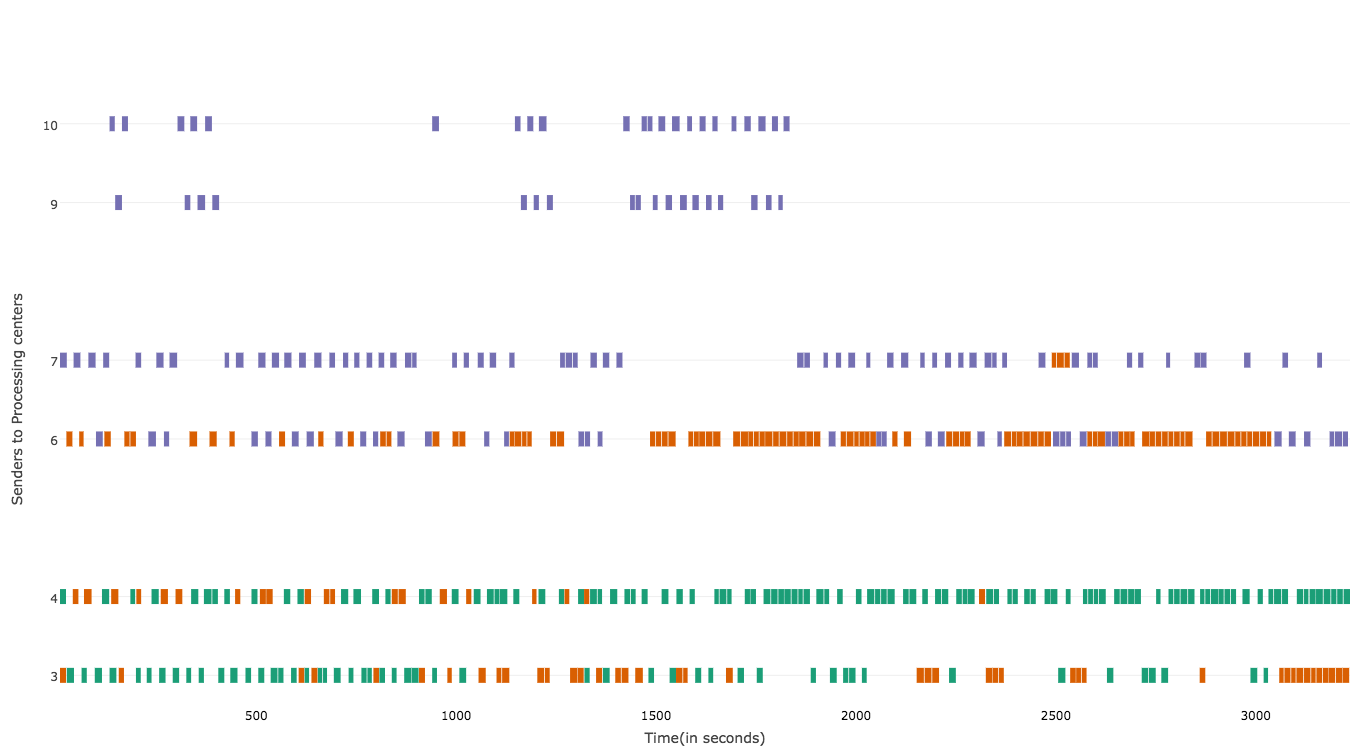
\includegraphics[width=1.0\textwidth]{gfx/RPlots/DFD_EllipsoidTopology.png}
    \caption{Data transfer schedule in heterogeneity: Ellipsoidal Topology}
    \label{fig:dfd_ellipsoid}
    \end{figure}
        
	\begin{figure}
    \centering
    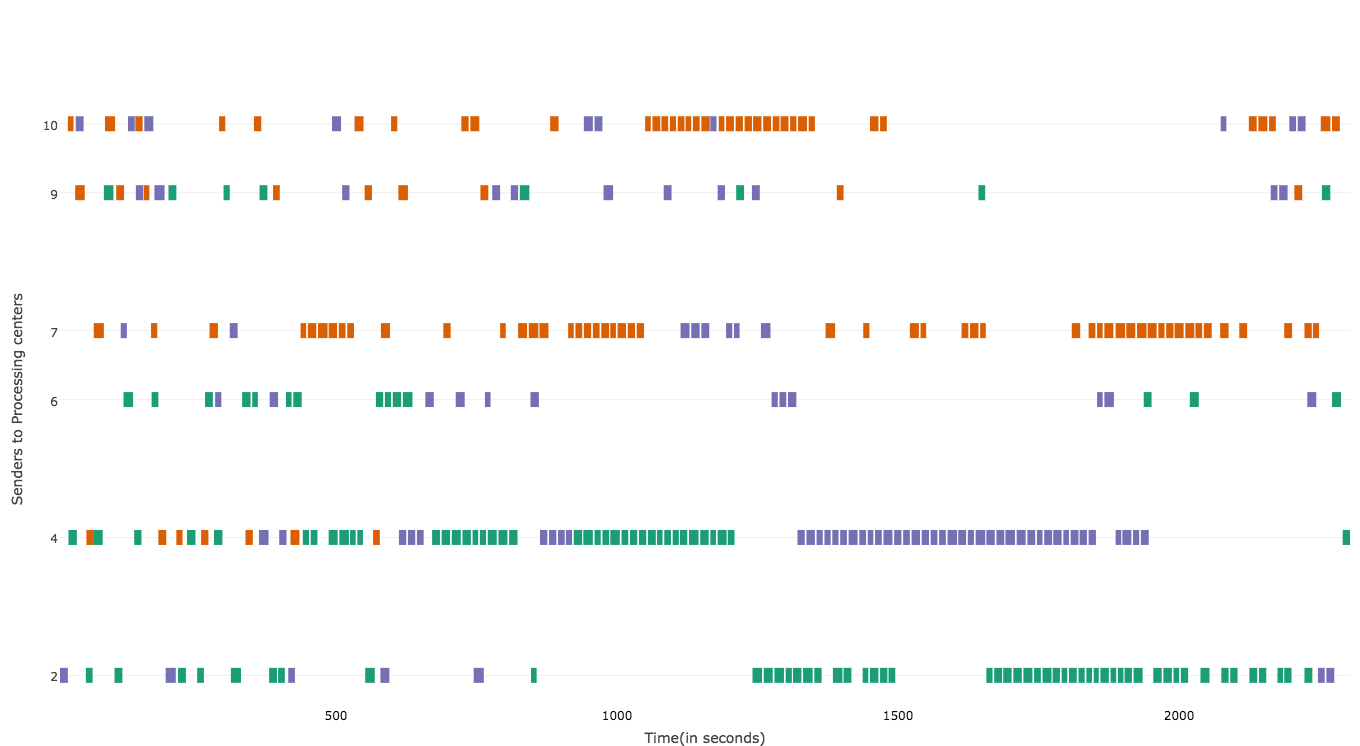
\includegraphics[width=1.0\textwidth]{gfx/RPlots/DFD_TreeTopology.png}
    \caption{Data transfer schedule in heterogeneity: Tree Topology}
    \label{fig:dfd_tree}
    \end{figure}
    
    From the following diagrams, we can infer the following regarding evaluation measures:
    
    \begin{enumerate}
        \item Sender Fairness: From the box plot diagram \ref{fig:boxplot_treeVsEllipsoid}, we can infer that \acp{PC} are more evenly distributed among intended senders in Tree topology than Ellipsoid topology because the contending senders have more fair chances to occupy \ac{PC} in former topology than the latter pattern. Also, for ellipsoid topology, most of the senders are either in two hop neighborhood of \acp{PC} or cannot occupy distant (more than two hop) \acp{PC} before the \ac{PC}'s immediate neighbor \ac{RTS}. Therefore, these senders have limited options of selecting a \ac{PC} for data transmission.
        
    	\begin{figure}
        \centering
        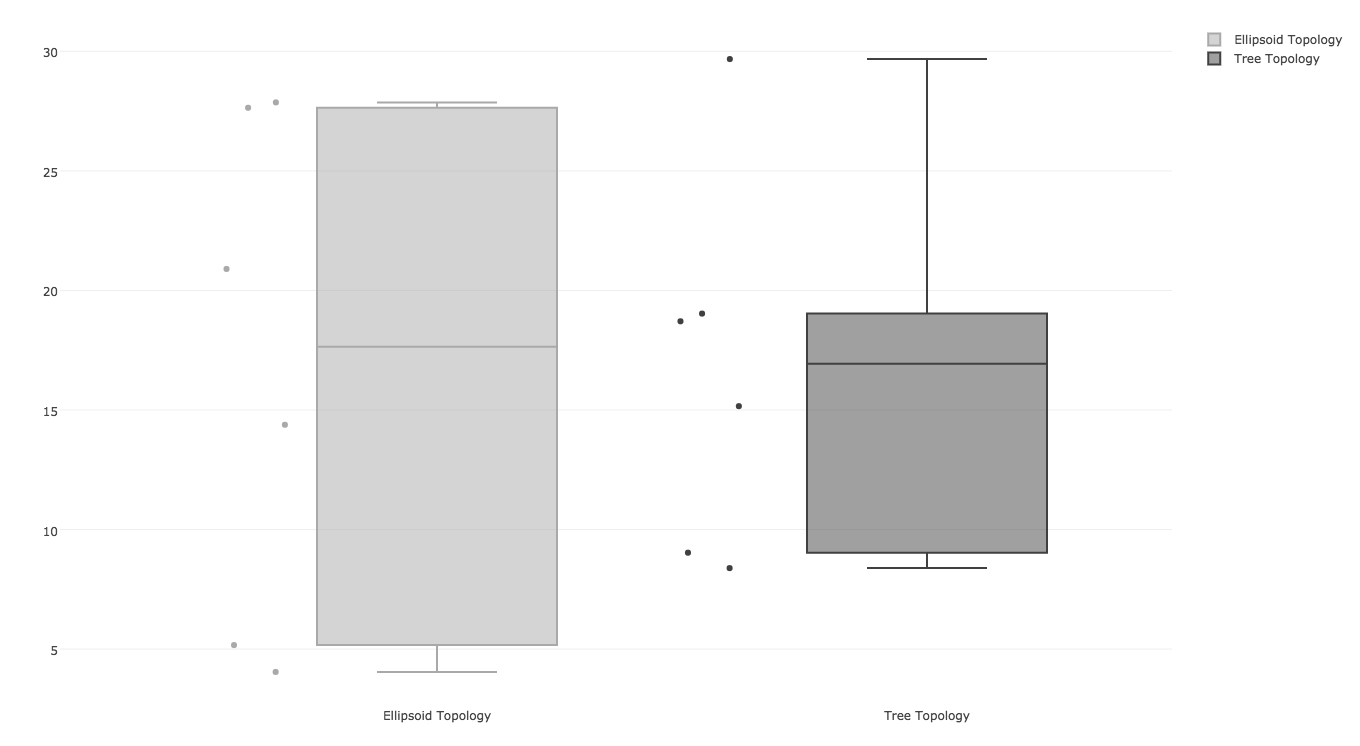
\includegraphics[width=1.0\textwidth]{gfx/RPlots/boxplot_senderFairnessComparison.png}
        \caption{Sender Fairness: Ellipsoid vs Tree Topology}
        \label{fig:boxplot_treeVsEllipsoid}
        \end{figure}
    
        \item Relayer Fairness: The two hop requests in both the topologies are not so frequent because of less chances to get \ac{CTS} response for a \ac{RTS} packet from a far away sender than the near by sender. This can be deduced from the figure \ref{fig:relayerFiarness}, in which the graph shows maximum for both the topologies when relayer address is zero (which means that the relayer is not used and rather one hop sending is used). There are two reasons for this phenomenon: 1. The time taken to reach two hop \ac{RTS} by a two hop sender is greater than the time taken to deliver one hop \ac{RTS} by one hop sender. 2. For a two hop request, the sender must first send in its \ac{RTS} request, a blocking signal for the relayer. This blocking is only confirmed when the relayer, which has to be blocked for the requested time slot, has not sent its \ac{RTS} request prior to the contending sender. The probability of occurrence for such an incidence is low because the \ac{PC} exists in the immediate neighborhood for the relayer than the contending two hop sender.
        
    	\begin{figure}
        \centering
        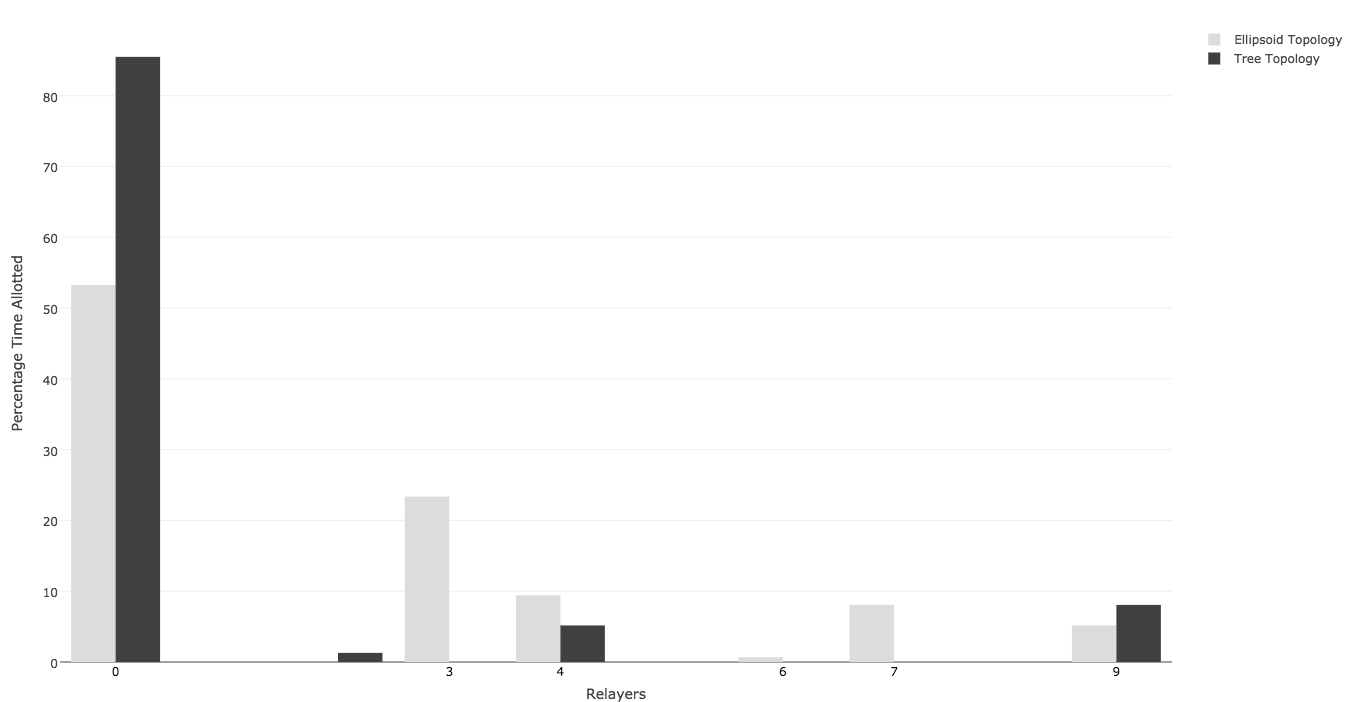
\includegraphics[width=1.0\textwidth]{gfx/RPlots/relayer_fairness.png}
        \caption{Relayer Fairness: Ellipsoid vs Tree Topology}
        \label{fig:relayerFiarness}
        \end{figure}
        
        \par        
        Also it can be inferred from the diagrams that relayers are used more often in ellipsoid topology as compared to tree topology. This happens because for each \ac{PC}, in ellipsoid topology, there can be maximum two contending \acp{SN} where as in the given tree topology there are more than two senders in one hop contending for a single \ac{PC}.
        
        \item \ac{PC} Occupancy: We ran the simulation four times for around seventy minutes and took the average of occupancy duration for each of the \acp{PC}. This reading is plotted in the figure \ref{fig:pcenterOccupancy}, where on $X$ axis the \acp{PC} are shown and on $Y$ axis we plot the percentage of time allotted out of the total simulation run time. It can be observed from the diagram that the \acp{PC} could not be kept occupied  100 percent of the simulation run time. This is because of the numerous \ac{RTS} and \ac{CTS} beacon exchanges and contention in the channel to make both \ac{CTP} and heterogeneity layer work for data transmissions. However, with the achieved \ac{PC} occupancy for about $50$ percent and more for each \ac{PC}, we are still able to achieve better performance than \ac{CTP} in terms of number of packets delivered at \ac{BS}. This is discussed in detail in the next subsection (\ref{subsec:prrlog}).
        
    	\begin{figure}
        \centering
        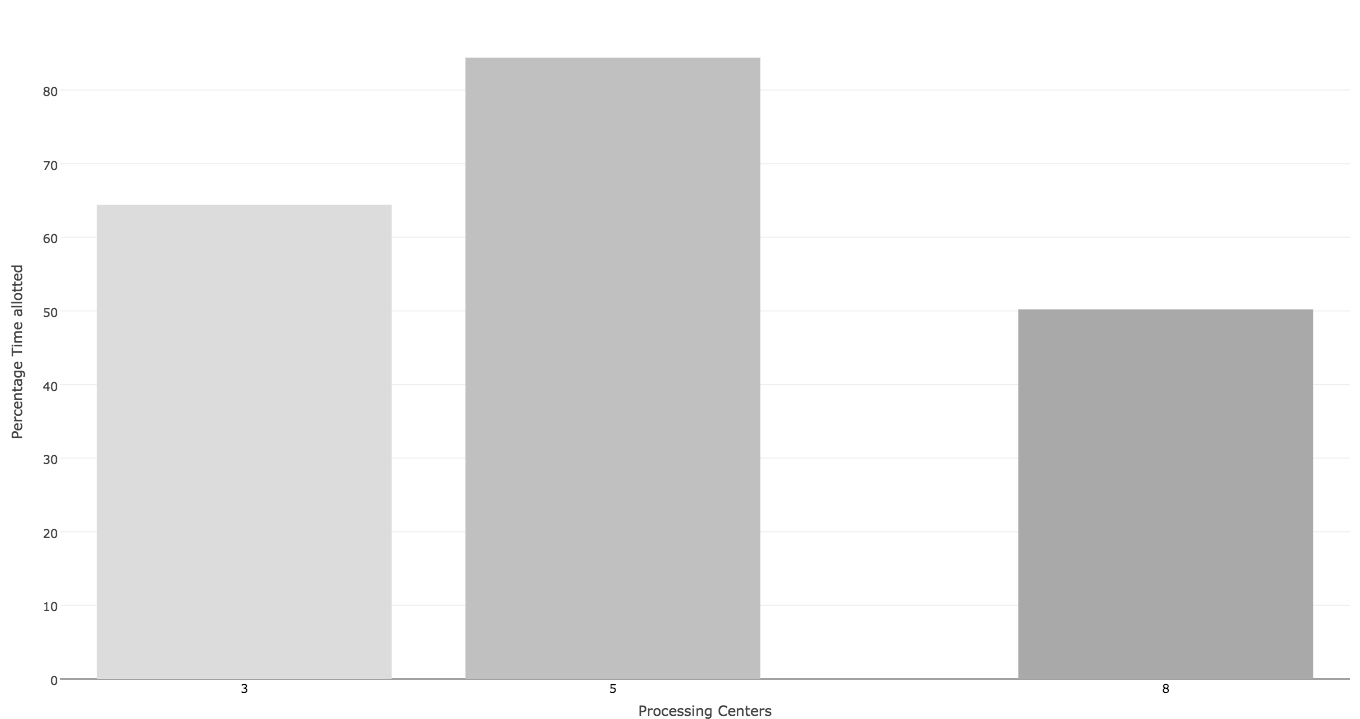
\includegraphics[width=1.0\textwidth]{gfx/RPlots/PCOccupancy.png}
        \caption{Processing Centre Occupancy}
        \label{fig:pcenterOccupancy}
        \end{figure}
        
    \end{enumerate}

	\begin{figure}
    \centering
    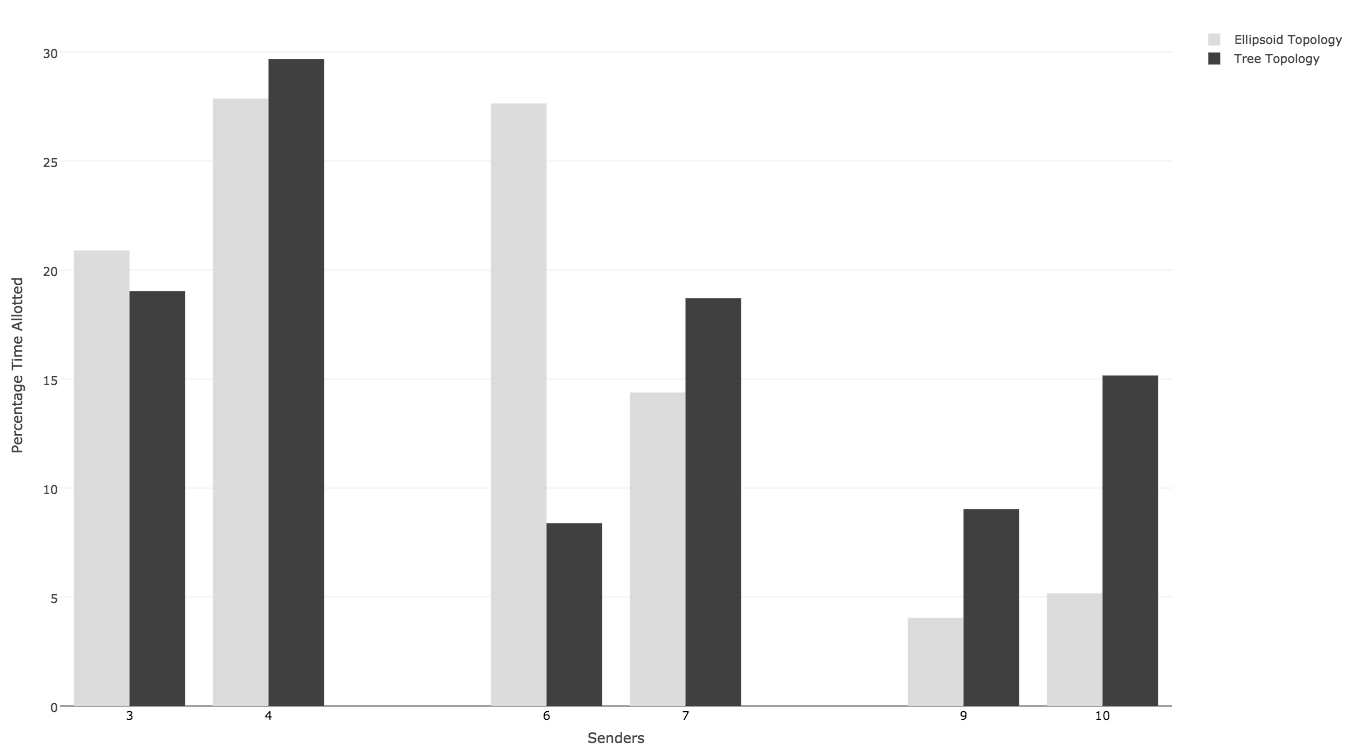
\includegraphics[width=1.0\textwidth]{gfx/RPlots/treevsellipsoid_fairness.png}
    \caption{Comparison: Ellipsoid vs Tree  Topology Sender Fairness}
    \label{fig:TreeVsEllipsoidTopology}
    \end{figure}
    
    %************************************************
    \subsection*{\ac{PRR} log}\label{subsec:prrlog}
    %************************************************
    
    This log stores list of packets sent and received by the intended \ac{SN} and \ac{PC} respectively. On every packet transmitted/received, total number of packets sent/received counter is incremented. After the sender runs out of allotted time, the counter is forwarded to the serial output and further displayed in the Cooja mote output window. The log file is further saved as \textit{.txt} file to analyse the packet reception ratio in heterogeneity.
    
    %************************************************
    \subsection*{PRR Log Analysis}
    %************************************************

    We use the above described log file to analyse following two scenarios. 
    
    \begin{enumerate}
        \item Analyse how \ac{PRR} changes on changing the heterogeneity data transmission period.
        
        \item Perform a comparative analysis of number of packets received by \ac{CTP} to number of packets received by heterogeneity at different data transfer rates
    \end{enumerate}
    
    
    \par 
    Scenario 1: The figure \ref{fig:PRRHeterogeneity} represents the data delivery ratio of heterogeneity layer to the \ac{PC} at different data sending rates. This diagram presents an interesting overview of heterogeneity data sending rate versus \ac{PC} \ac{PRR}. It can be concluded from the graph that if we send the packets at lower transmission intervals, say at $50ms$ or less, we loose more packets however the total number of packets received at the \ac{PC} increases, whereas if we increase the heterogeneity data transfer intervals, we see a rise in \ac{PRR} but overall number of packets received falls down. The increase in \ac{PRR} from $91$ percent to $95$ percent is mainly due to reduced heterogeneity data traffic on increasing the transmission interval. With lower transmission interval in heterogeneity layer, the total number of sent packets increases and therefore the sender node needs frequent channel access to transmit the data. However, the channel also has to be accessed by \ac{CTP} layer for route maintenance and updating and packets transmission. This is the main reason for packet loss. Also, the rise in \ac{PRR} is primarily due to the fact that on increasing the periodic interval of transmission channel access, we reduce the channel access contention.
    
    \par
    The graph also reaches the saturation point of around $95$ percent after crossing the $120ms$ transmission interval checkpoint. The flattening of curve beyond $120ms$ data transfer interval is mainly because of the following reasons:
        
        \begin{enumerate}
            \item \ac{CTP} layer at the back end contends with the heterogeneity layer to send its packets to the \ac{BS} for data transmission or to maintain the \ac{CTP} tree with frequent beacon exchange. 
            
            \item Given that a collection layer at the back end is prime necessity for periodic data collection of processed or unprocessed data, it is not possible to circumvent the collection layer to improve \ac{PRR}.
            
            \item Re-transmission of undelivered packets is not implemented in heterogeneity. This is because we do not aim to achieve $100$ percent \ac{PRR} and rather we aim to demonstrate the advantages of local data processing and thus reducing the overall network burden.
        \end{enumerate}
        
	\begin{figure}
    \centering
    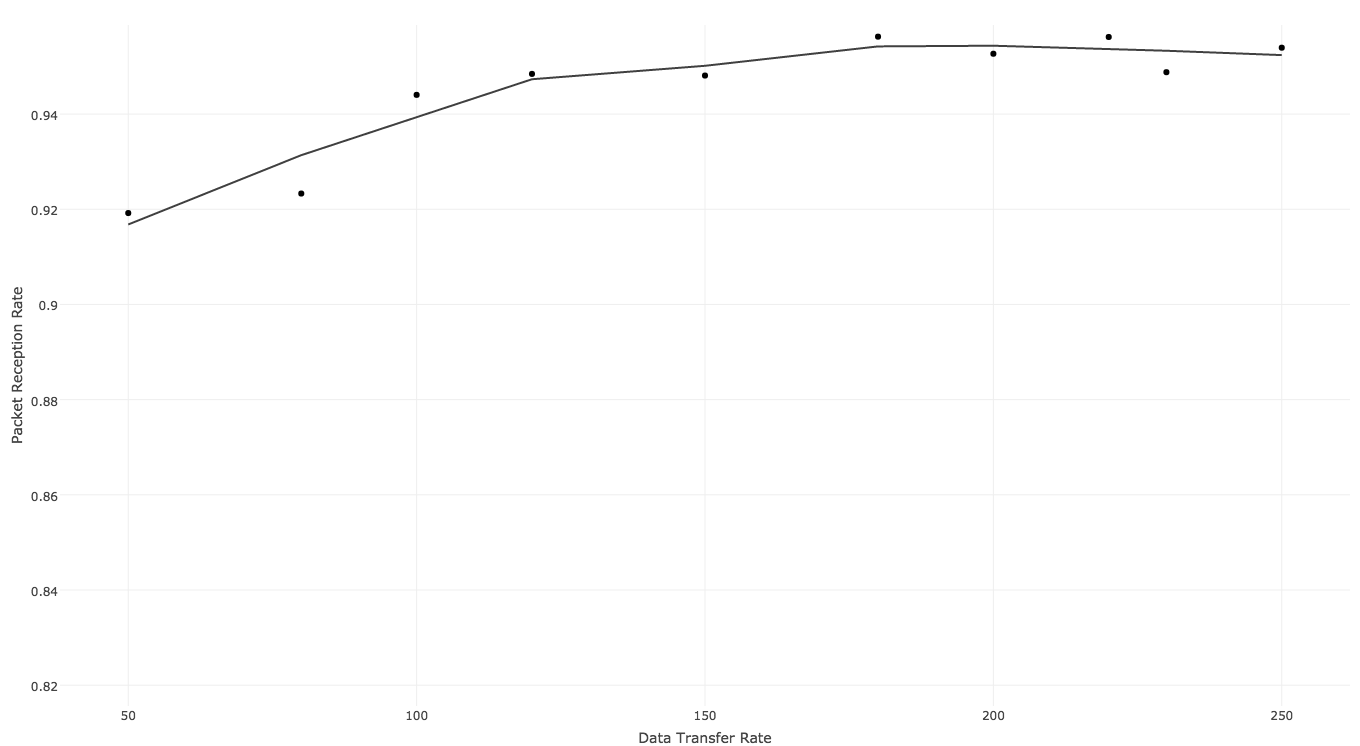
\includegraphics[width=1.0\textwidth]{gfx/RPlots/PrrVsDataTransferRate.png}
    \caption{PRR for different heterogeneity data transfer rates}
    \label{fig:PRRHeterogeneity}
    \end{figure}
    
    \par
    Second scenario: This study will demonstrate that a considerable amount of energy and time is saved by performing local computation at heterogeneous node. With this analysis, we also aim to show that heterogeneity reduces the burden of \ac{CTP} by a reasonable factor in carrying over the data generated at a \ac{SN} via the collection tree to the \ac{BS}. In order to perform the evaluation, we need to uniquely mark the data sent by heterogeneous processing point to distinguish it from unprocessed data and further on reception of a data at \ac{BS}, the counters for processed or unprocessed data is incremented based on the set or unset marker value respectively. 
    
    \par
    We show this comparison, in figure \ref{fig:DataProcessingHetvsCTP}, by plotting number of packets processed by heterogeneity to the number of packets collected via \ac{CTP} in twenty five minutes of Cooja simulation run time at several heterogeneity data transfer intervals. We represent data transfer rate at collection interval of $2000ms$ on $X$ axis and \ac{PRR} for the receiver (which is the \ac{PC}) on $Y$ axis. From the graph it can be inferred that the heterogeneity layer receive more data at lower data transfer rate. This is because of frequent call to packet sending interface to send the generated data from the intended data sender node. In the diagram, the plot also decreases gradually on increasing the data transmission period because of increased heterogeneity periodic data transmission interval. 
    
    \par
    In the figure \ref{fig:DataProcessingHetvsCTP}, the ratio of heterogeneity processed data to \ac{CTP} unprocessed data at $50ms$ data transfer interval is approximately $7:1$. The selection of $50ms$ data transfer interval has one big disadvantage: only $91$ percent of the data sent by sender node reaches the \ac{PC} (as shown in figure \ref{fig:PRRHeterogeneity}). We can therefore make a trade-off between data delivery ratio and amount of data processed by operating heterogeneity layer at data transfer rate of approximately $120ms$. This will not only give us about $95$ percent \ac{PRR} at \ac{PC} but also deliver around $3.5$ times more packets than the \ac{CTP} layer. This approach will also reduce the total number of packets flowing through the collection protocol (after the data has reached the destination \ac{PC}). This is because the data which has to be earlier sent to the \ac{BS} for processing is already now processed and instead of transmitting all the packets to \ac{BS}, we send only a few processed packets. 
    
    \begin{figure}
    \centering
    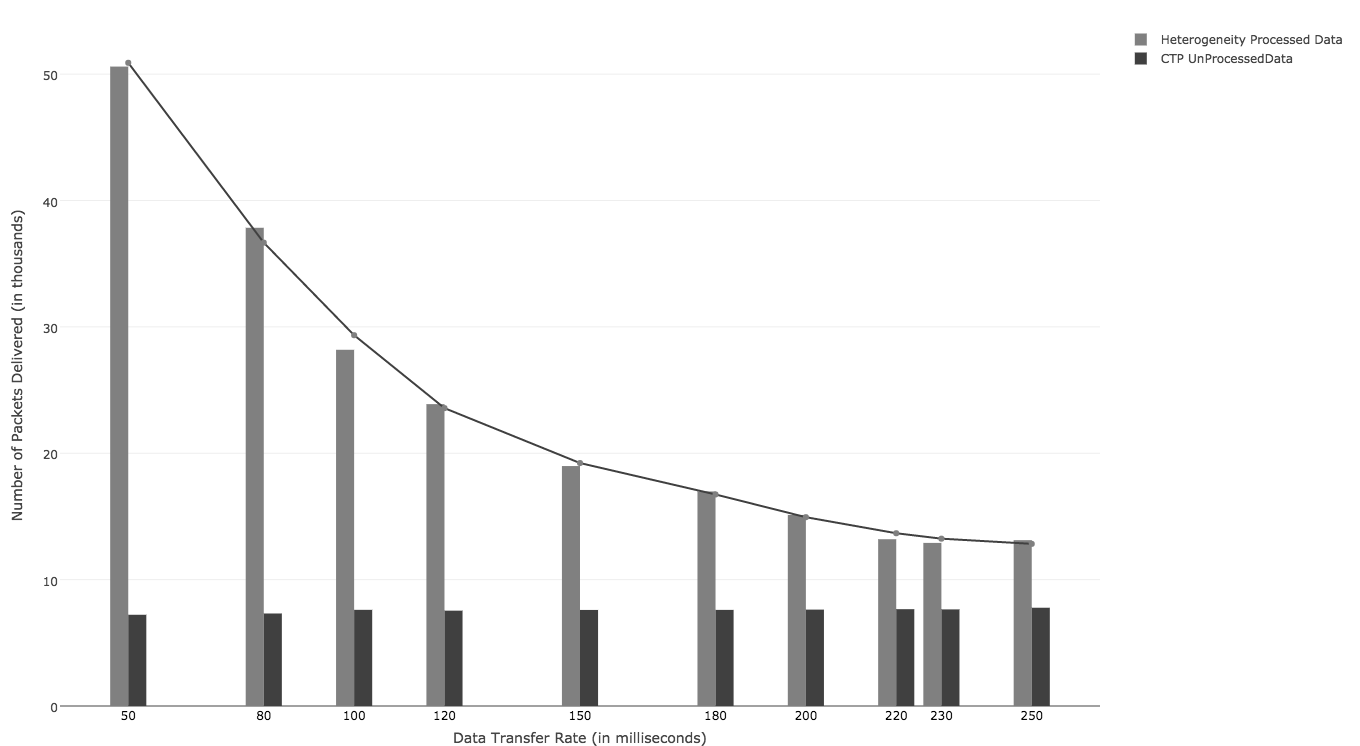
\includegraphics[width=1.0\textwidth]{gfx/RPlots/DataProcessingHetvsCTP.png}
    \caption{Comparison for number of packets delivered at \ac{BS} by heterogeneity vs CTP at varying data transfer rates}
    \label{fig:DataProcessingHetvsCTP}
    \end{figure}


%************************************************
\section{A Practical Overview of heterogeneity for Energy Efficiency}
%************************************************

To examine the energy efficiency of heterogeneity from a practical overview, let us assume that the \ac{PC} is five hops away from the \ac{BS} and the sender node is in two hop neighborhood of \ac{PC}. If  only the \ac{CTP} layer is active then the data generated at the \ac{SN} must travel seven hops to reach the \ac{BS} for getting processed. By the definition of a heterogeneous processing point, we can also assume that computation time is approximately same for both, heterogeneous node and \ac{BS}. We can see that the usual flow of large amount of data via \ac{CTP} not only burdens the entire network but also drains energy of the entire collection tree responsible for forwarding the data to the \ac{BS}. However, if we turn on the heterogeneity layer, then the data now only has to travel two hops and for the rest five hops the processed data is sent via \ac{CTP}. This approach saves energy of \acp{SN} participating in the collection tree, reduces the traffic flow in the sensor network and also allows heavy data traffic without burdening the entire \ac{WSN} except the participating nodes.
    
    % %************************************************
    % \subsection*{Energy Efficiency}
    % %************************************************


    
    
%     we set a uniform rate where there is a perfect trade off between data sending and reception rate and fix our data sending timer. After this we do a comparison study.
    

    
    
%     next evaluation is getting the data read by serial output port and further see how much we really process them and further demonstrate the computation time involved by giving the compute power to \ac{PC} through serial port to any device.
    
%     The evaluation on hardware 9independence will demonstrate that any serial device attached to the tmote is capable of processing the data... be it raspberripi or others....we also demonstrate that the code is compilable by all the \acp{SN}.

% %************************************************
% \section{Evaluation Goals}
% %************************************************

% In this section we will describe the  


        
%         (average \ac{PC} allocation time is 16seconds for intended senders )

% \begin{enumerate}
	
% 	\item Cluster-based: The processing centre is assigned to each group of cluster of \acp*{WSN} and the \acp*{SN} route using CTP tree routing.
	
% 	\item Tree-based: In this mechanism, some parents of the tree are Processing centres and others are either using CTP protocol to send the data or they use NFS-SIS scheme to send the data to their parents.
	
% 	\item Ellipsoidal: Nodes are arranged in ellipsoidical fashion, where some nodes in the ring are Processing centre.
	
% 	\item Random: Randomly distributing nodes in a network based on random location generated by Contiki for each \ac*{SN}
	
% \end{enumerate}

% In each of the above mentioned topological order of the nodes, the following parameters are evaluated:

% \section*{Energy Consumption}

% \begin{enumerate}
% 	\item Overall Energy Consumption: Energy dissipation of each sensor node. Plot for each \ac{SN} on 2D Cartesian axes, where X -> Time (In hrs) Y -> Energy(In Joules) 
	
% 	\item LifeCycle of a \ac{WSN}:
	
% 	\begin{enumerate}
% 		\item Time till first \ac{SN} dies on 2D Cartesian axes, where X -> Time (In hrs) Y -> Energy(In Joules) 
		
% 		\item Time till all \acp*{SN} dies		
% 	\end{enumerate}
	
% \end{enumerate}

% \section*{Energy Consumption}

% \begin{enumerate}
% 	\item Gantt Chart for each \ac*{SN} to show CTS-RTS time frame on time as X-axis
	
% 	\item Time when data delivery to BaseStation falls below a certain threshold
% \end{enumerate}

% \section*{Scalability}

% \begin{enumerate}
% 	\item Network Performance on increasing the number of nodes. Plot for each \ac*{SN} on 2D Cartesian axes, where X -> Number of SensorNodes Y -> Simulation running Speed in contiki
% \end{enumerate}

% \section*{Overheads and Efficiency}

% \begin{enumerate}
% 	\item Control Overhead: Number of Control Messages to Data Messages
% \end{enumerate}

% \section*{Other Evaluation Data}

% \begin{enumerate}
	
% 	\item Algorithm Storage requirement of \ac*{CTP} vs \ac*{NFS-SIS}
	
% 	\item Mobility of \acp*{SN} in \ac*{NFS-SIS}
	
% 	\item Performance ratio on $ Num SensorNodes \div Num ProcessingCentres $
	
	
% \end{enumerate}



% \par

% Qestions to be answered:

% Why don't we choose \ac{CTP} root node advertising scheme to send data to the \acp{PC} on the assumption that the \ac{PC} is a \ac{BS}. what drawbacks this scheme might have?